\documentclass{fdubeamer}

\usetikzlibrary{arrows.meta, calc, decorations.markings}
\tikzset{
  x = 1em,
  y = 1em,
  node font = \footnotesize,
  morphism box/.style = {draw, fill = white, anchor = base},
  tensor box/.style = {semithick, FudanRed, fill=FudanRed!30},
  tensor leg/.style = {semithick, MaterialGrey},
  covered tensor leg/.style = {semithick, dashed, MaterialGrey300},
  ->-/.style = {
    decoration = {
      markings,
      mark = at position #1 with {\arrow{Stealth}},
    },
    postaction = {decorate},
  },
}
\newcommand{\Tetrahedron}[6]{
  \begin{tikzpicture}[baseline=1ex]
    \draw [covered tensor leg, MaterialGrey] (0,0) -- (3.2,0);
    \draw [tensor leg]
          (0,0) -- (2,2.5) -- (3.2,0) -- (2,-0.8) -- cycle
          (2,2.5) -- (2,-0.8);
    \draw (0.6, 1.7) node {$#1$}
          (3.2, 1.7) node {$#2$}
          (0.6,-0.9) node {$#3$}
          (3  ,-0.9) node {$#4$}
          (1.1, 0.5) node {$#5$}
          (2.4, 0.8) node {$#6$};
  \end{tikzpicture}
}
\newcommand{\Triangle}[6]{
  \begin{tikzpicture}[baseline=-0.5ex]
    \draw [tensor box]
          ( 90:1.5) -- (210:1.5) -- (330:1.5) -- cycle;
    \foreach \x in {90, 210, 330}
      \draw [tensor leg]
          (\x-40:1.7) .. controls (\x-20:0.8) and (\x+20:0.8) .. (\x+40:1.7)
          (\x-60:0.4) -- (\x-60:1.6);
    \draw ( 30:2) node {$#1$}
          (150:2) node {$#2$}
          (270:2) node {$#3$}
          ( 90:2) node {$#4$}
          (210:2) node {$#5$}
          (330:2) node {$#6$};
  \end{tikzpicture}
}
\newcommand{\tikzinput}[1]{\input{includes/tikz/#1.tex}}
\newcommand{\1}{\mathbb{1}}
\NewDocumentCommand{\ket}{som}{%
  \IfBooleanTF{#1}{|#3\rangle}{%
    \IfValueTF{#2}{#2|#3#2\rangle}{\left|#3\right\rangle}}}

\title{Aspects on Tensor Networks for Topological Orders}
\author{Xiangdong Zeng}
\institute{Supervisor: Prof.\ Ling-Yan Hung}
% \date{\today}

\begin{document}

\maketitle

\begin{frame}{Outline}

\begin{itemize}
  \item Motivation and background

    \begin{itemize}
      \item AdS/CFT correspondence
      \item Topological orders and category theory
      \item Tensor networks
    \end{itemize}

  \item Strange correlators and holographic tensor networks

    \begin{itemize}
      \item Tensor network representation of string-net model
      \item Strange correlators and MPO symmetries
      \item Construction of holographic tensor networks
      \item Operator pushing
    \end{itemize}

  \item Tensor network representations of Virasoro and Kac--Moody algebra

    \begin{itemize}
      \item Review of 2d CFT
      \item Basic construction
      \item Examples: Ising, dimer and Fibonacci models
    \end{itemize}
\end{itemize}

\end{frame}

\section{Motivation \& background}

\begin{frame}{Motivation: AdS/CFT correspondence}

\begin{columns}[c]

  \column{0.6\textwidth}

    \begin{itemize}
      \item Duality between a gravity theory in AdS\textsubscript{\textit{d}+1} spacetime (bulk) and a CFT\textsubscript{\textit{d}+1} (boundary)
      \item AdS/CFT dictionary: $Z_{\mathrm{CFT}}=Z_{\mathrm{bulk}}$
      \item Ryu--Takayanagi formula:

        \begin{itemize}
          \item $S_A = \operatorname{Area}(\gamma_A) / 4G^{(d+1)}$
          \item Entanglement is geometry
        \end{itemize}

      \item AdS/CFT and machine learning

        \begin{itemize}
          \item Mapping to Boltzmann machine
          \item CNN as RG flow
        \end{itemize}

      \item \textit{p}-adic AdS/CFT and Einstein equation
    \end{itemize}

  \column{0.4\textwidth}

    \centering
    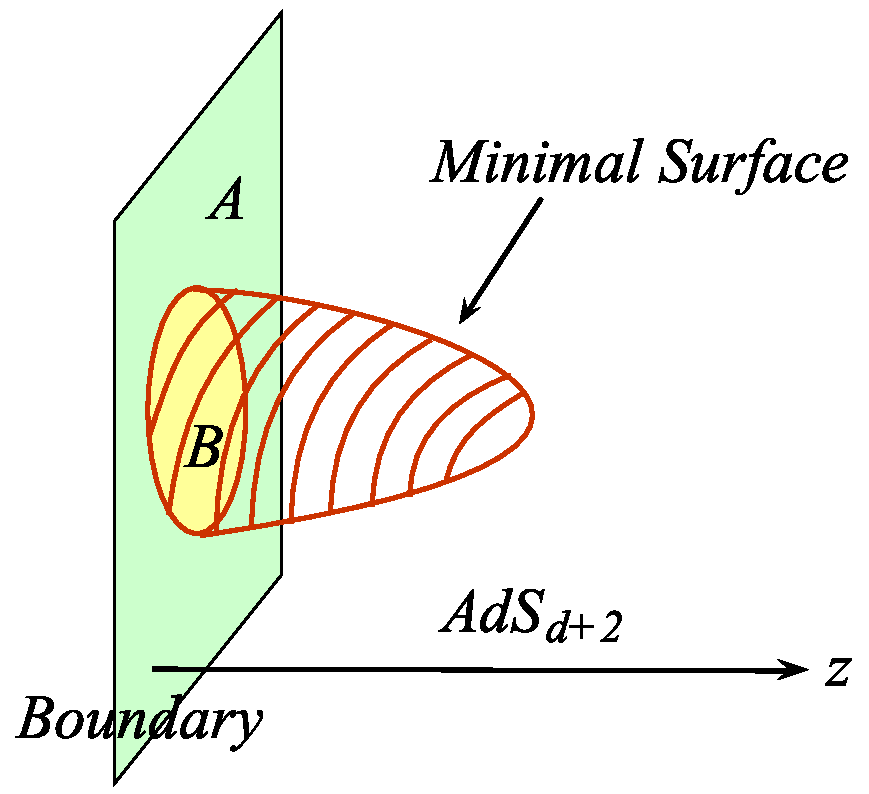
\includegraphics[width=0.8\textwidth]{images/rt-formula.pdf}

\end{columns}

\footnotetext{Image credit: \citet{nishioka2009holographic}}

\end{frame}

\begin{frame}{Topological orders}

\begin{itemize}
  \item Novel phases of matter beyond Landau's theory

    \begin{itemize}
      \item Fractional quantum Hall effect
      \item High temperature superconductivity
    \end{itemize}

  \item Fundamental properties:

    \begin{itemize}
      \item Ground state degeneracy
      \item Non-Abelian geometric phase
    \end{itemize}

  \item Microscopic origin:

    \begin{itemize}
      \item Long-range entanglement
      \item Local unitary transformation
    \end{itemize}

  \item Applications: fault-tolerant quantum computation
  \item Mathematical framework: modular tensor categories (fusion categories)
\end{itemize}

\end{frame}

\begin{frame}{Tensor \& fusion categories}

\begin{itemize}
  \item Tensor product: $\otimes$

    \begin{itemize}
      \item Associativity: $(a\otimes b)\otimes c=a\otimes(b\otimes c)$
      \item Unit object: $\1\otimes a=a\otimes\1=a$
    \end{itemize}

  \item Simple objects and their fusion: $a\otimes b=\bigoplus_c N_{ab}^c c$

    \begin{itemize}
      \item Simple objects $a,b$: different types of anyon
      \item Fusion: can't be distinguished at long distance
      \item Fusion coefficients: $N_{ab}^c\in\mathbb{Z}^*$
      \item Quantum dimension $d_a$: max eigenvalue of matrix $(N_a)_{bc}=N_{ab}^c$
    \end{itemize}

  \item Examples:

    \begin{itemize}
      \item Decomposition of direct product of group representations
      \item Operator product expansion (OPE) in CFT
    \end{itemize}

  \item More structures: dual, braiding, ribbon, non-degeneracy, etc.
\end{itemize}

\end{frame}

\begin{frame}{Fusion diagrams}

\linespread{1.4}
\selectfont

\begin{columns}[c]

  \column{0.6\textwidth}

    \begin{itemize}
      \item Basis in vector space $\operatorname{Hom}_{\mathcal{C}}(a\otimes b,c)$:
            {\small \tikzinput{category/fusion-tree-1}}
      \item \textit{F}-move:
            {\small $\tikzinput{category/f-symbol-1} = \sum_y \, \bigl[ F^{abc}_d \bigr]_{xy} \tikzinput{category/f-symbol-2}$}
      \item Constraints: pentagon equations
      \item Bubble removal:
            \mbox{\qquad}{\small $\tikzinput{category/loop-removal}$}
    \end{itemize}

  \column{0.4\textwidth}

    \centering
    {\small \tikzinput{category/f-symbols-pentagon-equation-narrow}}

\end{columns}

\end{frame}

\begin{frame}{Examples of fusion categories}

\linespread{1.4}
\selectfont

\begin{itemize}
  \item Fibonacci

    \begin{itemize}
      \item Anyon types: $\{\1, \tau\}$
      \item Fusion rules: $\tau\otimes\tau=\1\oplus\tau$
      \item Quantum dimensions: $d_{\1}=1, \, d_\tau=\varphi$
      \item \textit{F}-symbols:
        $
          [F^{\tau\tau\tau}_\tau]_{ij} = \frac{1}{\varphi} \Bigl(\begin{smallmatrix} 1 & \sqrt\varphi \\ \sqrt\varphi & -1 \end{smallmatrix}\Bigr), \,
          i,j \in \{\1, \tau\}
        $
    \end{itemize}

  \item Ising

    \begin{itemize}
      \item Anyon types: $\{\1, \sigma, \psi\}$
      \item Fusion rules: $\psi\otimes\psi=\1, \, \sigma\otimes\sigma=\1\oplus\psi, \, \psi\otimes\sigma=\sigma$
      \item Quantum dimensions: $d_{\1}=d_\psi=1, \, d_\sigma=\sqrt2$
      \item \textit{F}-symbols:
        $
          [F^{\psi\sigma\psi}_\sigma]_{\sigma\sigma} = [F^{\sigma\psi\sigma}_\psi]_{\sigma\sigma} = -1, \,
          [F^{\sigma\sigma\sigma}_\sigma]_{ij} = -\frac{1}{\sqrt2} \Bigl(\begin{smallmatrix} 1 & 1 \\[0.5ex] 1 & -1 \end{smallmatrix}\Bigr), \,
          i,j \in \{\1, \psi\}
        $
    \end{itemize}
\end{itemize}

\end{frame}

\begin{frame}{String-net model}

\begin{itemize}
  \item Input data

    \begin{itemize}
      \item Trivalent lattice (e.g.\ honeycomb)
      \item Superselection sector (edge): simple objects
      \item Branching rules (vertex): fusion rules
    \end{itemize}

  \item Hamiltonian: $H = -\sum_v A_v - \sum_p B_p$

    \begin{itemize}
      \item Electric charge:
        $A_v \, \ket[\Bigg]{\tikzinput{string-net/fusion-2}} = \delta_{ijk} \, \ket[\Bigg]{\tikzinput{string-net/fusion-2}}$
      \item Magnetic flux:
        $B_p = \sum_{s=0}^N \frac{d_s}{D^2} B_p^s \, , \quad D = \sqrt{\sum_{s=0}^N d_s^2}$ \\
        $
            \phantom{\text{Magnetic flux:~}}
            B_p^s \, \ket[\Bigg]{\def\Prime{}\tikzinput{string-net/hexagon}}
          = \sum_{m,\dots,r} B_{p,ghijkl}^{s,g'h'i'j'k'l'} \,
            \ket[\Bigg]{\def\Prime{'}\tikzinput{string-net/hexagon}}
        $
    \end{itemize}
\end{itemize}

\end{frame}

\begin{frame}{Tensor networks}

\begin{columns}[c]

  \column{0.6\textwidth}

    \begin{itemize}
      \item Tensor: a multi-dimensional array
      \item Contraction and decomposition (SVD)
      \item Why efficient?

        \begin{itemize}
          \item Only keep the relevant (i.e.\ entanglement) degrees of freedom
          \item Area-law: $S\sim\partial A$
        \end{itemize}

      \item Algorithms:

        \begin{itemize}
          \item MPS/MPO based: DMRG, TEBD, etc.

            \begin{itemize}
              \item 2d generalization: PEPS/PEPO
            \end{itemize}

          \item Coarse-graining: TRG, TNR, HOTRG, etc.
          \item MERA: holographic geometry
        \end{itemize}
    \end{itemize}

  \column{0.4\textwidth}

    \centering
    \tikzinput{tensor-network/tensor-networks}

\end{columns}

\footnotetext{Image credit: \citet{orus2019tensor} (with modification)}

\end{frame}

\section{Strange correlators \& \\ holographic tensor networks}

\begin{frame}{Tensor network representation of string-net model}

\begin{columns}[c]

  \column{0.5\textwidth}

    \begin{itemize}
      \item Construct ground state: is given by 

        \begin{itemize}
          \item Apply $B_p$ on vacuum state $\ket{\diameter}$
          \item Weighted by quantum dimensions
          \item Use \textit{F}-moves to simplify
        \end{itemize}

      \item PEPS structure:

        \begin{itemize}
          \item Virtual indices: summed over \\
            \mbox{\qquad} (outside two legs: $\alpha,\beta,\gamma$)
          \item Physical indices: left uncontracted
            \mbox{\qquad} (inner one leg: $i,j,k$)
        \end{itemize}

      \item Tetrahedral symmetry: $A_4$ group
    \end{itemize}

  \column{0.5\textwidth}

    \centering
    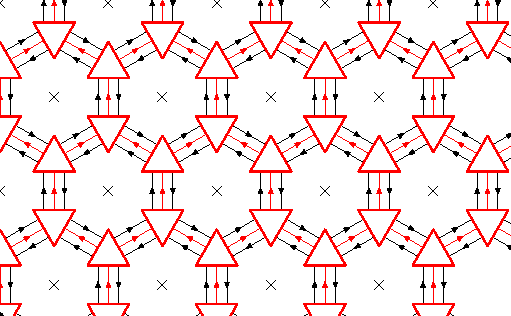
\includegraphics[width=0.7\textwidth]{images/string-net-peps.pdf}
    \begingroup
      \scriptsize
      \setlength{\arraycolsep}{1.5pt}
      \tikzset{x=1em, y=1em, node font=\tiny}
      \begin{gather*}
          \Triangle jki\alpha\beta\gamma
        = \frac{1}{D} (d_i d_j d_k)^{-\frac14} (d_\alpha d_\beta d_\gamma)^{-\frac13}
          \Tetrahedron ik\gamma\alpha\beta j \\
          \bigl[ F^{abc}_d \bigr]_{xy}
        = \sqrt{d_x d_y} \begin{bmatrix} a & b & x\, \\ c & d & y\, \end{bmatrix}
        = \frac{1}{\sqrt{d_a d_b d_c d_d}} \, \Tetrahedron xbdyca
      \end{gather*}
    \endgroup
    \vspace*{-4em}

\end{columns}

\footnotetext{Image credit: \citet{buerschaper2009explicit}}

\end{frame}

\begin{frame}{Strange correlators}

\end{frame}

\section{Tensor network representations of \\ Virasoro \& Kac--Moody algebra}

\begin{frame}{References}
  \tiny
  \bibliography{main}
\end{frame}

\begingroup
  \setbeamercolor{background canvas}{bg=FudanBlue}
  \begin{frame}[plain]
    \vfill
    \begin{center}
      \color{white}
      \LARGE
      \textbf{Thank you!} \par
      \vspace{6em}
      \tiny
      \copyright{} 2023 Xiangdong Zeng
    \end{center}
    \vspace{-8em}
  \end{frame}
\endgroup

\end{document}
